% !TEX root = main.tex

\section{存储与文件结构} % Chap 10
\subsection{存储器件}
物理存储:易失(volatile)、非易失

磁盘被划分为道、扇区、柱面

常见磁盘性能衡量指标:
\begin{itemize}
	\item 访问时间:
	\begin{itemize}
		\item 寻道(seek)时间:到达特定的道
		\item 旋转时间
	\end{itemize}
	\item 数据传输速率
	\item 平均失效时间(MTTF):通常3-5年
\end{itemize}

通过并行来提高性能:数据拆分(striping)
\begin{itemize}
	\item 比特级拆分:每个字节按比特分开,存储到多个磁盘上
	\item 块级拆分:将块拆分到多张磁盘,即将磁盘阵列看成一张单独的大磁盘,并给块进行逻辑编号
\end{itemize}

独立磁盘冗余阵列(Redundant Array of Independent Disk, RAID)

\begin{minipage}[H]{0.5\linewidth}
\begin{itemize}
	\item RAID-0:块级拆分但无冗余
	\item RAID-1:块级拆分+冗余,数据库常用
	\item RAID-2:纠错码(Error-Correcting-Code, ECC),可以读出其余位和纠错位重建信息
	\item RAID-3:可以检测一整个扇区是否被正确读出
	\item RAID-4:在一张独立磁盘上为其他$N$张磁盘对应的块保留一个奇偶校验块
	\item RAID-5:将数据和奇偶校验位分布到$N+1$张磁盘中,所有磁盘都能参与读请求
	\item RAID-6:P+Q冗余方案,可应对多张磁盘故障情况
\end{itemize}
\end{minipage}
\begin{minipage}[H]{0.5\linewidth}
\begin{figure}[H]
\centering
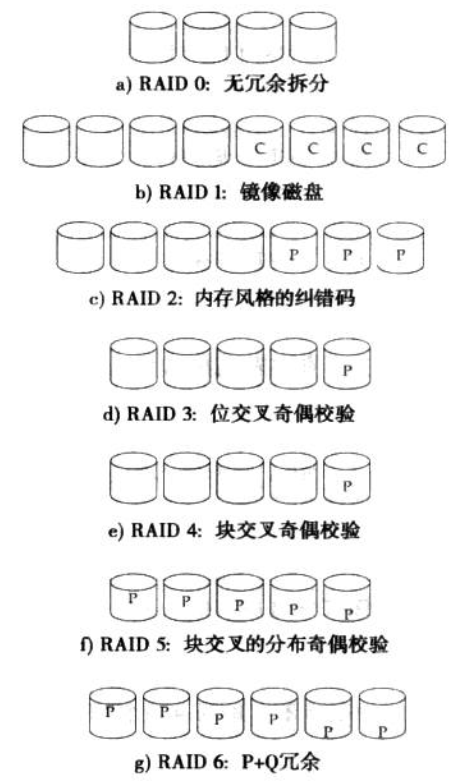
\includegraphics[width=0.5\linewidth]{fig/RAID.png}
\end{figure}
\end{minipage}

\subsection{文件结构}
\subsubsection{定长记录}
每次插入删除都涉及后续元组的移动,可以如下维护一个空闲列表(free list)
\begin{figure}[H]
\centering
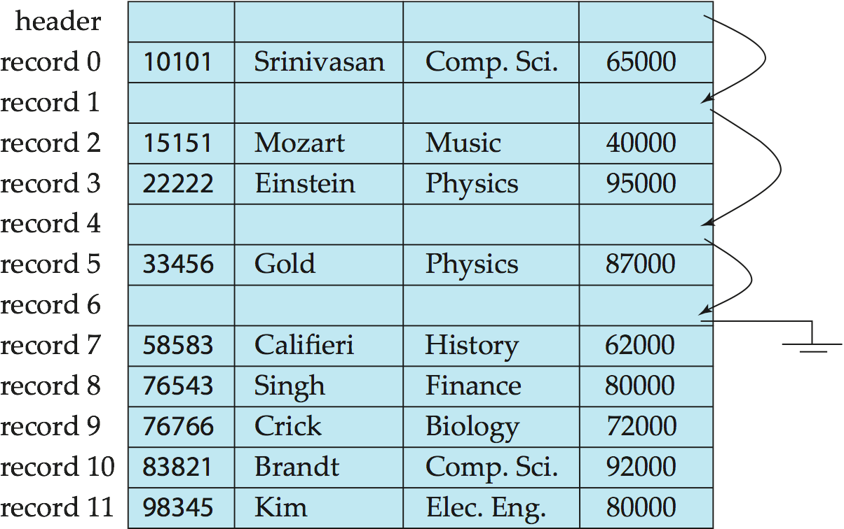
\includegraphics[width=0.6\linewidth]{fig/free_lists.png}
\end{figure}

\subsubsection{变长记录}
变长记录以以下几种方式出现:
\begin{itemize}
	\item 多种记录类型在一个文件中存储
	\item 允许一个或多个字段是变长的记录类型
	\item 允许可重复字段的记录类型,如数组或多重集合
\end{itemize}
\begin{figure}[H]
\centering
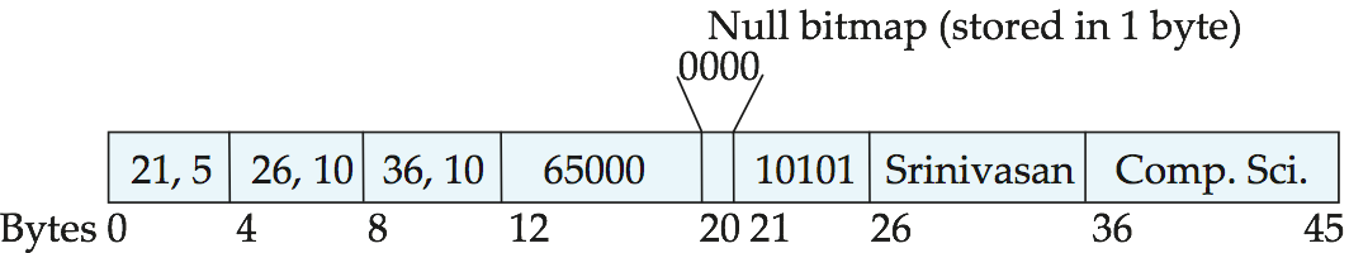
\includegraphics[width=0.5\linewidth]{fig/variable-length.png}
\end{figure}

用分槽的页结构(slotted-page)来处理块中变长记录的问题
\begin{figure}[H]
\centering
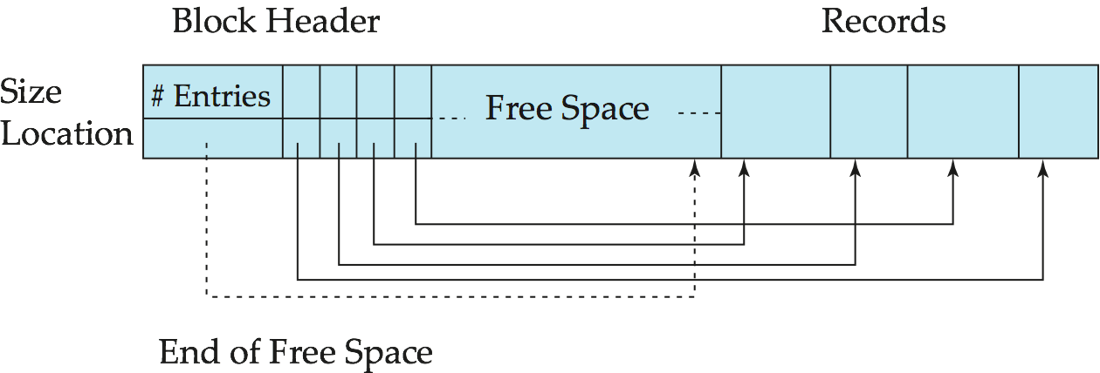
\includegraphics[width=0.5\linewidth]{fig/slotted_page.png}
\end{figure}

块头包含以下信息
\begin{itemize}
	\item 块头中记录条目的个数
	\item 块中空闲空间的末尾处
	\item 由包含记录位置和大小的记录条目组成的数组
\end{itemize}
注意实际记录是从\textemph{块的尾部}往前插。

\subsection{文件中记录的组织}
\begin{itemize}
	\item 堆文件组织:一条记录可放在文件中任何地方,只要那个地方有空间存放这条记录
	\item 顺序文件组织:根据其搜索码值顺序存储
	\item 散列文件组织:散列函数
\end{itemize}

多表聚簇组织
\begin{figure}[H]
\centering
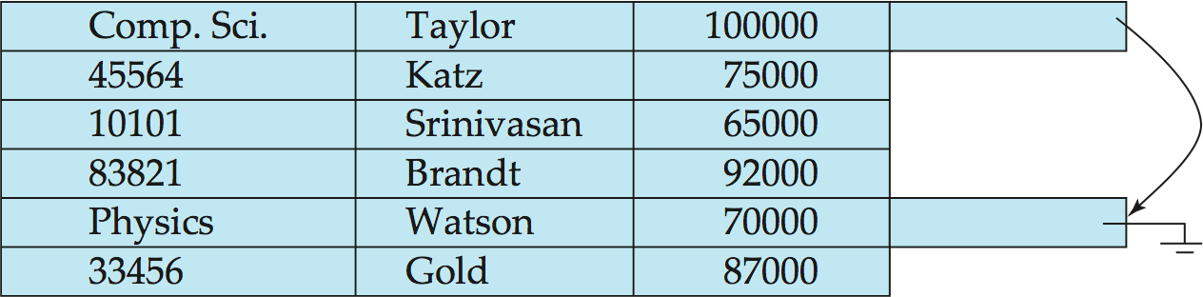
\includegraphics[width=0.5\linewidth]{fig/multitable_clustering.png}
\end{figure}